% =====================================================================
% SETUP DE HARDWARE (Metodologia) -- rascunho de 2026-11-04
% Ainda não incluído no METODOLOGIA.tex. Para incluir:
%   \section{Hardware Setup}\label{sec:setup-hardware}
%   % =====================================================================
% SETUP DE HARDWARE (Metodologia) -- rascunho de 2026-11-04
% Ainda não incluído no METODOLOGIA.tex. Para incluir:
%   \section{Hardware Setup}\label{sec:setup-hardware}
%   % =====================================================================
% SETUP DE HARDWARE (Metodologia) -- rascunho de 2026-11-04
% Ainda não incluído no METODOLOGIA.tex. Para incluir:
%   \section{Hardware Setup}\label{sec:setup-hardware}
%   % =====================================================================
% SETUP DE HARDWARE (Metodologia) -- rascunho de 2026-11-04
% Ainda não incluído no METODOLOGIA.tex. Para incluir:
%   \section{Hardware Setup}\label{sec:setup-hardware}
%   \input{chapters/METODOLOGIA/setup-hardware.tex}
% Fontes do projeto (conferidas em 2026-11-04):
%   hardware/pacote_servidor_formatos/{LEIAME.md, vivado.tcl, potencia.py, rodar.sh}
%   hardware/pacote_servidor_2023/LEIAME.md
%   hardware/testes/{AMOSTRAGEM.md, LEIAME.md}
%   hardware/cholesky_hardware/{hls_config_sintese_24_12*.cfg, tb_potencia.cpp}
%   hardware/cholesky_hardware_diretivas*/LEIAME.md; acompanhamento_experimentos.csv
% Nomes das configurações: mapa LETRAS de software/testes/mapa_cenarios_v4.py
%   (antigos 1-8 = 1A,1E,1B,1F,1C,1G,1D,1H; 9-12 = 2A,2E,2B,2F).
% =====================================================================

% ---------------------------------------------------------------------
\subsection{\texorpdfstring{Tools and target device}{Tools and target device}}\label{subsec:hw-ferramentas}
% ---------------------------------------------------------------------
The inversion module was described in C++ and synthesized in Vitis HLS 2026.1. Vitis HLS generates the module's RTL. Then, the RTL was synthesized, placed, and routed in Vivado 2023.2. The target device is the AMD Alveo U50 board, with the XCU50-FSVH2104-2-E FPGA. This FPGA has 5,952 DSP blocks and 871,680 LUTs. All circuits use a clock frequency of 100 MHz, or a period of 10 ns.

In Vivado, the inversion module is synthesized and implemented alone, as the top-level design, without any other surrounding board logic. The flow performs synthesis, optimization, placement, physical optimization, and routing. The only timing constraint is the clock period, and the paths entering and exiting the module's ports are not constrained. Thus, the resource, timing, and power figures for this work are only for the module and come from the routed design in Vivado 2023.2.

Before the Vivado workflow, each version went through the Vitis HLS C synthesis. A version only went to Vivado if the HLS estimate fit within the FPGA: a maximum of 5,952 DSP blocks and a maximum of 90\% of the LUTs.

% ---------------------------------------------------------------------
\subsection{\texorpdfstring{Inversion module}{Inversion module}}\label{subsec:hw-modulo}
% ---------------------------------------------------------------------
The module receives the $M_c \times M_c$ matrix $\mathbf{G}_c$ and returns its inverse. It calculates the inverse using Cholesky decomposition (Section~\ref{sec:inversao}). Two sizes for $\mathbf{G}_c$, corresponding to the configurations described in Section~\ref{subsec:configuracoes-bs}, have been implemented: $16 \times 16$ and $32 \times 32$. The input, output, and internal values use the \texttt{ap\_fixed} data type, following the formats selected in Section~\ref{sec:formato}.

The module consists of six stages, each implemented as a C++ function (Figure~\ref{fig:modulo-inversao}). These stages are executed sequentially, with each stage passing its output to the next.
\begin{figure}[!ht]
\caption{Steps of the inversion module. Each block is one C++ function of the HLS code.}
\label{fig:modulo-inversao}
\vspace{4pt} % a classe zera o espaço entre a caption e a figura
\centering
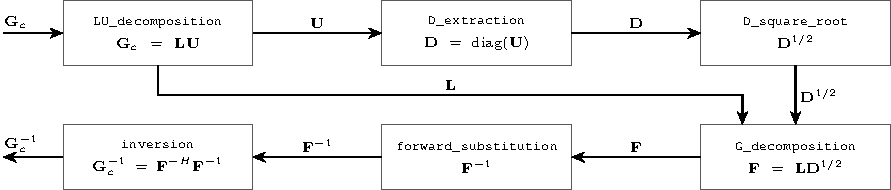
\includegraphics{Images/FLUXO/modulo_inversao.pdf}
\vspace{4pt}
\legend{Source: the author.}
\end{figure}

Additions, multiplications, and divisions utilize \texttt{ap\_fixed} type operators. Complex multiplication and division operations are explicitly implemented in the code, with a specific type defined for each intermediate value; thus, the bit-width of every intermediate value is explicitly set within the code. The addition of two $N$-bit numbers requires $N+1$ bits, while their product requires $2N$ bits \cite[pp.~72--73]{kastner-hls}. When using \texttt{ap\_fixed} types, the result of an operation inherently possesses a sufficient number of bits; overflow only occurs when this result is assigned to a type with a smaller bit-width \cite[p.~74]{kastner-hls}. Consequently, intermediate values employ types with greater bit-widths than the $\langle W, I\rangle$ format (Table~\ref{tab:tipos-intermediarios}), with the result reverting to the specified format only at the output of each stage. Square root calculations are performed using the \texttt{hls::sqrt} function from Vitis HLS, operating directly within the defined format.

\begin{table}[!ht]
\caption{Types of the values in the inversion module, for the format $\langle W, I\rangle$ with $F = W - I$ fractional bits.}
\label{tab:tipos-intermediarios}
\vspace{4pt} % a classe zera o espaço entre a caption e a tabela
\centering
\footnotesize
\renewcommand{\arraystretch}{1.2}
\begin{tabular}{p{7.4cm}cc}
\toprule
\textbf{Value} & \textbf{Integer bits} & \textbf{Fractional bits} \\
\midrule
Input, output and output of each step & $I$ & $F$ \\
Square root (\texttt{hls::sqrt}) & $I$ & $F$ \\
Accumulated sums, numerator and divisor of the complex division, quotient & $2I$ & $2F$ \\
Product of two real numbers & $4I$ & $4F$ \\
Real or imaginary part of a complex product (sum of two products) & $4I + 1$ & $4F$ \\
\bottomrule
\end{tabular}
\vspace{4pt}
\legend{Source: the author. The intermediate values use the same quantization and overflow modes as the format; the square root uses AP\_TRN and AP\_WRAP.}
\end{table}


% ---------------------------------------------------------------------

% Fontes do projeto (conferidas em 2026-11-04):
%   hardware/pacote_servidor_formatos/{LEIAME.md, vivado.tcl, potencia.py, rodar.sh}
%   hardware/pacote_servidor_2023/LEIAME.md
%   hardware/testes/{AMOSTRAGEM.md, LEIAME.md}
%   hardware/cholesky_hardware/{hls_config_sintese_24_12*.cfg, tb_potencia.cpp}
%   hardware/cholesky_hardware_diretivas*/LEIAME.md; acompanhamento_experimentos.csv
% Nomes das configurações: mapa LETRAS de software/testes/mapa_cenarios_v4.py
%   (antigos 1-8 = 1A,1E,1B,1F,1C,1G,1D,1H; 9-12 = 2A,2E,2B,2F).
% =====================================================================

% ---------------------------------------------------------------------
\subsection{\texorpdfstring{Tools and target device}{Tools and target device}}\label{subsec:hw-ferramentas}
% ---------------------------------------------------------------------
The inversion module was described in C++ and synthesized in Vitis HLS 2026.1. Vitis HLS generates the module's RTL. Then, the RTL was synthesized, placed, and routed in Vivado 2023.2. The target device is the AMD Alveo U50 board, with the XCU50-FSVH2104-2-E FPGA. This FPGA has 5,952 DSP blocks and 871,680 LUTs. All circuits use a clock frequency of 100 MHz, or a period of 10 ns.

In Vivado, the inversion module is synthesized and implemented alone, as the top-level design, without any other surrounding board logic. The flow performs synthesis, optimization, placement, physical optimization, and routing. The only timing constraint is the clock period, and the paths entering and exiting the module's ports are not constrained. Thus, the resource, timing, and power figures for this work are only for the module and come from the routed design in Vivado 2023.2.

Before the Vivado workflow, each version went through the Vitis HLS C synthesis. A version only went to Vivado if the HLS estimate fit within the FPGA: a maximum of 5,952 DSP blocks and a maximum of 90\% of the LUTs.

% ---------------------------------------------------------------------
\subsection{\texorpdfstring{Inversion module}{Inversion module}}\label{subsec:hw-modulo}
% ---------------------------------------------------------------------
The module receives the $M_c \times M_c$ matrix $\mathbf{G}_c$ and returns its inverse. It calculates the inverse using Cholesky decomposition (Section~\ref{sec:inversao}). Two sizes for $\mathbf{G}_c$, corresponding to the configurations described in Section~\ref{subsec:configuracoes-bs}, have been implemented: $16 \times 16$ and $32 \times 32$. The input, output, and internal values use the \texttt{ap\_fixed} data type, following the formats selected in Section~\ref{sec:formato}.

The module consists of six stages, each implemented as a C++ function (Figure~\ref{fig:modulo-inversao}). These stages are executed sequentially, with each stage passing its output to the next.
\begin{figure}[!ht]
\caption{Steps of the inversion module. Each block is one C++ function of the HLS code.}
\label{fig:modulo-inversao}
\vspace{4pt} % a classe zera o espaço entre a caption e a figura
\centering
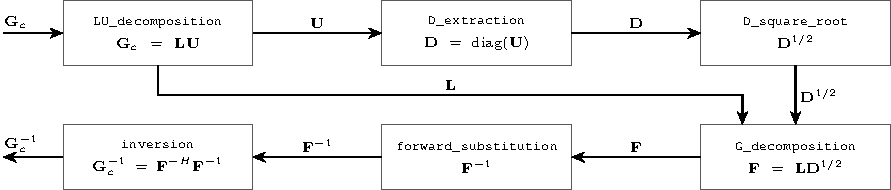
\includegraphics{Images/FLUXO/modulo_inversao.pdf}
\vspace{4pt}
\legend{Source: the author.}
\end{figure}

Additions, multiplications, and divisions utilize \texttt{ap\_fixed} type operators. Complex multiplication and division operations are explicitly implemented in the code, with a specific type defined for each intermediate value; thus, the bit-width of every intermediate value is explicitly set within the code. The addition of two $N$-bit numbers requires $N+1$ bits, while their product requires $2N$ bits \cite[pp.~72--73]{kastner-hls}. When using \texttt{ap\_fixed} types, the result of an operation inherently possesses a sufficient number of bits; overflow only occurs when this result is assigned to a type with a smaller bit-width \cite[p.~74]{kastner-hls}. Consequently, intermediate values employ types with greater bit-widths than the $\langle W, I\rangle$ format (Table~\ref{tab:tipos-intermediarios}), with the result reverting to the specified format only at the output of each stage. Square root calculations are performed using the \texttt{hls::sqrt} function from Vitis HLS, operating directly within the defined format.

\begin{table}[!ht]
\caption{Types of the values in the inversion module, for the format $\langle W, I\rangle$ with $F = W - I$ fractional bits.}
\label{tab:tipos-intermediarios}
\vspace{4pt} % a classe zera o espaço entre a caption e a tabela
\centering
\footnotesize
\renewcommand{\arraystretch}{1.2}
\begin{tabular}{p{7.4cm}cc}
\toprule
\textbf{Value} & \textbf{Integer bits} & \textbf{Fractional bits} \\
\midrule
Input, output and output of each step & $I$ & $F$ \\
Square root (\texttt{hls::sqrt}) & $I$ & $F$ \\
Accumulated sums, numerator and divisor of the complex division, quotient & $2I$ & $2F$ \\
Product of two real numbers & $4I$ & $4F$ \\
Real or imaginary part of a complex product (sum of two products) & $4I + 1$ & $4F$ \\
\bottomrule
\end{tabular}
\vspace{4pt}
\legend{Source: the author. The intermediate values use the same quantization and overflow modes as the format; the square root uses AP\_TRN and AP\_WRAP.}
\end{table}


% ---------------------------------------------------------------------

% Fontes do projeto (conferidas em 2026-11-04):
%   hardware/pacote_servidor_formatos/{LEIAME.md, vivado.tcl, potencia.py, rodar.sh}
%   hardware/pacote_servidor_2023/LEIAME.md
%   hardware/testes/{AMOSTRAGEM.md, LEIAME.md}
%   hardware/cholesky_hardware/{hls_config_sintese_24_12*.cfg, tb_potencia.cpp}
%   hardware/cholesky_hardware_diretivas*/LEIAME.md; acompanhamento_experimentos.csv
% Nomes das configurações: mapa LETRAS de software/testes/mapa_cenarios_v4.py
%   (antigos 1-8 = 1A,1E,1B,1F,1C,1G,1D,1H; 9-12 = 2A,2E,2B,2F).
% =====================================================================

% ---------------------------------------------------------------------
\subsection{\texorpdfstring{Tools and target device}{Tools and target device}}\label{subsec:hw-ferramentas}
% ---------------------------------------------------------------------
The inversion module was described in C++ and synthesized in Vitis HLS 2026.1. Vitis HLS generates the module's RTL. Then, the RTL was synthesized, placed, and routed in Vivado 2023.2. The target device is the AMD Alveo U50 board, with the XCU50-FSVH2104-2-E FPGA. This FPGA has 5,952 DSP blocks and 871,680 LUTs. All circuits use a clock frequency of 100 MHz, or a period of 10 ns.

In Vivado, the inversion module is synthesized and implemented alone, as the top-level design, without any other surrounding board logic. The flow performs synthesis, optimization, placement, physical optimization, and routing. The only timing constraint is the clock period, and the paths entering and exiting the module's ports are not constrained. Thus, the resource, timing, and power figures for this work are only for the module and come from the routed design in Vivado 2023.2.

Before the Vivado workflow, each version went through the Vitis HLS C synthesis. A version only went to Vivado if the HLS estimate fit within the FPGA: a maximum of 5,952 DSP blocks and a maximum of 90\% of the LUTs.

% ---------------------------------------------------------------------
\subsection{\texorpdfstring{Inversion module}{Inversion module}}\label{subsec:hw-modulo}
% ---------------------------------------------------------------------
The module receives the $M_c \times M_c$ matrix $\mathbf{G}_c$ and returns its inverse. It calculates the inverse using Cholesky decomposition (Section~\ref{sec:inversao}). Two sizes for $\mathbf{G}_c$, corresponding to the configurations described in Section~\ref{subsec:configuracoes-bs}, have been implemented: $16 \times 16$ and $32 \times 32$. The input, output, and internal values use the \texttt{ap\_fixed} data type, following the formats selected in Section~\ref{sec:formato}.

The module consists of six stages, each implemented as a C++ function (Figure~\ref{fig:modulo-inversao}). These stages are executed sequentially, with each stage passing its output to the next.
\begin{figure}[!ht]
\caption{Steps of the inversion module. Each block is one C++ function of the HLS code.}
\label{fig:modulo-inversao}
\vspace{4pt} % a classe zera o espaço entre a caption e a figura
\centering
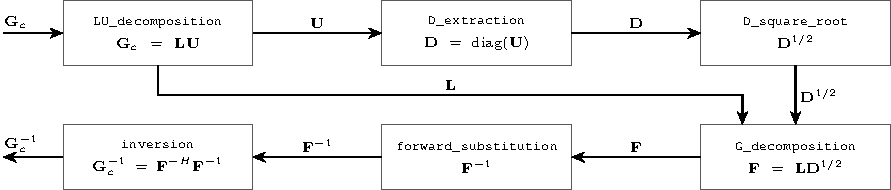
\includegraphics{Images/FLUXO/modulo_inversao.pdf}
\vspace{4pt}
\legend{Source: the author.}
\end{figure}

Additions, multiplications, and divisions utilize \texttt{ap\_fixed} type operators. Complex multiplication and division operations are explicitly implemented in the code, with a specific type defined for each intermediate value; thus, the bit-width of every intermediate value is explicitly set within the code. The addition of two $N$-bit numbers requires $N+1$ bits, while their product requires $2N$ bits \cite[pp.~72--73]{kastner-hls}. When using \texttt{ap\_fixed} types, the result of an operation inherently possesses a sufficient number of bits; overflow only occurs when this result is assigned to a type with a smaller bit-width \cite[p.~74]{kastner-hls}. Consequently, intermediate values employ types with greater bit-widths than the $\langle W, I\rangle$ format (Table~\ref{tab:tipos-intermediarios}), with the result reverting to the specified format only at the output of each stage. Square root calculations are performed using the \texttt{hls::sqrt} function from Vitis HLS, operating directly within the defined format.

\begin{table}[!ht]
\caption{Types of the values in the inversion module, for the format $\langle W, I\rangle$ with $F = W - I$ fractional bits.}
\label{tab:tipos-intermediarios}
\vspace{4pt} % a classe zera o espaço entre a caption e a tabela
\centering
\footnotesize
\renewcommand{\arraystretch}{1.2}
\begin{tabular}{p{7.4cm}cc}
\toprule
\textbf{Value} & \textbf{Integer bits} & \textbf{Fractional bits} \\
\midrule
Input, output and output of each step & $I$ & $F$ \\
Square root (\texttt{hls::sqrt}) & $I$ & $F$ \\
Accumulated sums, numerator and divisor of the complex division, quotient & $2I$ & $2F$ \\
Product of two real numbers & $4I$ & $4F$ \\
Real or imaginary part of a complex product (sum of two products) & $4I + 1$ & $4F$ \\
\bottomrule
\end{tabular}
\vspace{4pt}
\legend{Source: the author. The intermediate values use the same quantization and overflow modes as the format; the square root uses AP\_TRN and AP\_WRAP.}
\end{table}


% ---------------------------------------------------------------------

% Fontes do projeto (conferidas em 2026-11-04):
%   hardware/pacote_servidor_formatos/{LEIAME.md, vivado.tcl, potencia.py, rodar.sh}
%   hardware/pacote_servidor_2023/LEIAME.md
%   hardware/testes/{AMOSTRAGEM.md, LEIAME.md}
%   hardware/cholesky_hardware/{hls_config_sintese_24_12*.cfg, tb_potencia.cpp}
%   hardware/cholesky_hardware_diretivas*/LEIAME.md; acompanhamento_experimentos.csv
% Nomes das configurações: mapa LETRAS de software/testes/mapa_cenarios_v4.py
%   (antigos 1-8 = 1A,1E,1B,1F,1C,1G,1D,1H; 9-12 = 2A,2E,2B,2F).
% =====================================================================

% ---------------------------------------------------------------------
\subsection{\texorpdfstring{Tools and target device}{Tools and target device}}\label{subsec:hw-ferramentas}
% ---------------------------------------------------------------------
The inversion module was described in C++ and synthesized in Vitis HLS 2026.1. Vitis HLS generates the module's RTL. Then, the RTL was synthesized, placed, and routed in Vivado 2023.2. The target device is the AMD Alveo U50 board, with the XCU50-FSVH2104-2-E FPGA. This FPGA has 5,952 DSP blocks and 871,680 LUTs. All circuits use a clock frequency of 100 MHz, or a period of 10 ns.

In Vivado, the inversion module is synthesized and implemented alone, as the top-level design, without any other surrounding board logic. The flow performs synthesis, optimization, placement, physical optimization, and routing. The only timing constraint is the clock period, and the paths entering and exiting the module's ports are not constrained. Thus, the resource, timing, and power figures for this work are only for the module and come from the routed design in Vivado 2023.2.

Before the Vivado workflow, each version went through the Vitis HLS C synthesis. A version only went to Vivado if the HLS estimate fit within the FPGA: a maximum of 5,952 DSP blocks and a maximum of 90\% of the LUTs.

% ---------------------------------------------------------------------
\subsection{\texorpdfstring{Inversion module}{Inversion module}}\label{subsec:hw-modulo}
% ---------------------------------------------------------------------
The module receives the $M_c \times M_c$ matrix $\mathbf{G}_c$ and returns its inverse. It calculates the inverse using Cholesky decomposition (Section~\ref{sec:inversao}). Two sizes for $\mathbf{G}_c$, corresponding to the configurations described in Section~\ref{subsec:configuracoes-bs}, have been implemented: $16 \times 16$ and $32 \times 32$. The input, output, and internal values use the \texttt{ap\_fixed} data type, following the formats selected in Section~\ref{sec:formato}.

The module consists of six stages, each implemented as a C++ function (Figure~\ref{fig:modulo-inversao}). These stages are executed sequentially, with each stage passing its output to the next.
\begin{figure}[!ht]
\caption{Steps of the inversion module. Each block is one C++ function of the HLS code.}
\label{fig:modulo-inversao}
\vspace{4pt} % a classe zera o espaço entre a caption e a figura
\centering
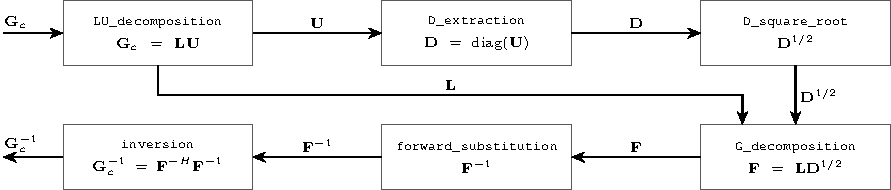
\includegraphics{Images/FLUXO/modulo_inversao.pdf}
\vspace{4pt}
\legend{Source: the author.}
\end{figure}

Additions, multiplications, and divisions utilize \texttt{ap\_fixed} type operators. Complex multiplication and division operations are explicitly implemented in the code, with a specific type defined for each intermediate value; thus, the bit-width of every intermediate value is explicitly set within the code. The addition of two $N$-bit numbers requires $N+1$ bits, while their product requires $2N$ bits \cite[pp.~72--73]{kastner-hls}. When using \texttt{ap\_fixed} types, the result of an operation inherently possesses a sufficient number of bits; overflow only occurs when this result is assigned to a type with a smaller bit-width \cite[p.~74]{kastner-hls}. Consequently, intermediate values employ types with greater bit-widths than the $\langle W, I\rangle$ format (Table~\ref{tab:tipos-intermediarios}), with the result reverting to the specified format only at the output of each stage. Square root calculations are performed using the \texttt{hls::sqrt} function from Vitis HLS, operating directly within the defined format.

\begin{table}[!ht]
\caption{Types of the values in the inversion module, for the format $\langle W, I\rangle$ with $F = W - I$ fractional bits.}
\label{tab:tipos-intermediarios}
\vspace{4pt} % a classe zera o espaço entre a caption e a tabela
\centering
\footnotesize
\renewcommand{\arraystretch}{1.2}
\begin{tabular}{p{7.4cm}cc}
\toprule
\textbf{Value} & \textbf{Integer bits} & \textbf{Fractional bits} \\
\midrule
Input, output and output of each step & $I$ & $F$ \\
Square root (\texttt{hls::sqrt}) & $I$ & $F$ \\
Accumulated sums, numerator and divisor of the complex division, quotient & $2I$ & $2F$ \\
Product of two real numbers & $4I$ & $4F$ \\
Real or imaginary part of a complex product (sum of two products) & $4I + 1$ & $4F$ \\
\bottomrule
\end{tabular}
\vspace{4pt}
\legend{Source: the author. The intermediate values use the same quantization and overflow modes as the format; the square root uses AP\_TRN and AP\_WRAP.}
\end{table}


% ---------------------------------------------------------------------
